% Chapter 3, Topic _Linear Algebra_ Jim Hefferon
%  http://joshua.smcvt.edu/linalg.html
%  2001-Jun-12
\topic{Line of Best Fit}
\index{least squares|(}
\index{line of best fit|(}
\index{linear equation!inconsistent systems}
\textit{This Topic requires the formulas from the subsections on 
        Orthogonal Projection Into a Line and Projection Into a
        Subspace.} 

Scientists are often presented with a system that 
has no solution and they must find an answer anyway. 
More precisely, they must
find a best answer.

For instance, 
this is the result of flipping a penny, including some
intermediate numbers.
\begin{center} \small
  \begin{tabular}{r|ccc}
     \textit{number of flips}  &30  &60  &90   \\
     \hline
     \textit{number of heads}  &16  &34  &51
  \end{tabular}
\end{center}
% In an experiment we expect that samples will vary. 
Here, sometimes
the experimental ratio of heads to flips  
overestimates this penny's long-term ratio of 50-50
and sometimes it underestimates.
So we expect that the system derived from the experiment has no solution. 
\begin{equation*}
  \begin{linsys}{1}
    30m  &=  &16    \\
    60m  &=  &34    \\
    90m  &=  &51
  \end{linsys}
\end{equation*}
That is, the vector of data that we collected is not in the subspace
where theory has it.
\begin{equation*}
  \colvec{16 \\ 34 \\ 51}\not\in
    \set{ m\colvec{30 \\ 60 \\ 90}  \suchthat m\in\Re}
\end{equation*}
However, we have to do something so we look for the~$m$ that most nearly works.
An orthogonal projection of the data vector into the line subspace
gives this best guess.
\begin{equation*}
  \frac{ \colvec[r]{16 \\ 34 \\ 51}\dotprod\colvec[r]{30 \\ 60 \\ 90} }{
           \colvec[r]{30 \\ 60 \\ 90}\dotprod\colvec[r]{30 \\ 60 \\ 90} }
     \cdot\colvec[r]{30 \\ 60 \\ 90}
  =\frac{7110}{12600}\cdot \colvec[r]{30 \\ 60 \\ 90}
\end{equation*}
The estimate (\( m=7110/12600\approx 0.56 \)) is a bit more than one half,
but not much more than half, 
so probably the penny is fair enough. 

The line with the slope \( m\approx 0.56 \)
is the \definend{line of best fit}\index{line!best fit}%
\index{best fit line} 
for this data.
\begin{center}  \small
  \includegraphics{ch3.42}
\end{center}
Minimizing the distance
between the given vector and the vector used as the right-hand side
minimizes the total of these vertical lengths,
and consequently
we say that the line comes from
\definend{fitting by least-squares}\index{least squares}
\begin{center}  \small
  \includegraphics{ch3.43}
\end{center}
(we have exaggerated the vertical scale by ten
to make the lengths visible).

In the above equation the line 
must pass through \( (0,0) \),
because we take it to be
the line whose slope is this coin's true proportion
of heads to flips. 
We can also handle cases where the line need not
pass through the origin.

Here is
the progression of world record times for the men's mile race \cite{Oakley}.
In the early 1900's many people wondered when, or if, 
this record would fall below the four minute mark.
Here are the times that were in force on January first
of each decade through the first half of that century.
\begin{center} \small
  \begin{tabular}{r|ccccccccc}
    \textit{year} &$1870$ &$1880$ &$1890$  &$1900$  
        &$1910$  &$1920$  &$1930$ &$1940$ &$1950$   \\
    \hline
    \textit{secs}  &$268.8$  &$264.5$  &$258.4$  &$255.6$  
        &$255.6$  &$252.6$  &$250.4$ &$246.4$ &$241.4$
  \end{tabular}  
\end{center}
We can use this to give a circa 1950 prediction of the date for $240$ seconds, 
and then compare that to the actual date.
(There are different sequences of times from competing standards
bodies but these are from \cite{WikipediaMensMile}.
Restricting to the times at the start of 
each decade reduces the data entry burden, smooths the data to some extent, 
and gives much the same result as entering all of the dates and records.)

As with the penny data, these numbers do not line in a perfect line.
That is, this system does not have an exact solution for the slope
and intercept.
\begin{equation*}
  \begin{linsys}{2}
    b &+  &1870m  &=  &268.8 \\ 
    b &+  &1880m  &=  &264.5 \\ 
      &   &       &\vdots     \\
    b &+  &1950m  &=  &241.4  
  \end{linsys}
\end{equation*}
We find a best approximation by using orthogonal projection.
Write the linear system's matrix of coefficients amd also its
vector of constants, the world record times.
\begin{equation*}
  A=
  \begin{mat}
    1  &1870  \\
    1  &1880  \\
    \vdots  &\vdots \\
    1  &1950  
  \end{mat}
  \qquad
  \vec{v}=\colvec{268.8 \\ 264.5 \\ \vdots \\ 241.4}
\end{equation*}
The ending result in the subsection on Projection into a Subspace 
gives the formula for the $b$ and $m$ so that the linear combination
of the columns of $A$ is as close as possible to the vector $\vec{v}$. 
They are the entries of 
the vector $(\trans{A}A)^{-1}\trans{A}\cdot\vec{v}$.

%\begin{center}
%  \begin{tabular}{r|ccccccc}
%    \textit{year} &1870  &1880  &1890  &1900  &1910  &1920  &1930   \\
%    \hline
%    \textit{seconds}  &$268.8$  &$264.5$  &$258.4$  &$255.6$  
%        &$255.6$  &$252.6$  &$250.4$
%  \end{tabular}        \\[2ex]
%  \begin{tabular}{|ccccccc}
%      1940  &1950  &1960  &1970  &1980  &1990 &2000                  \\
%      \hline
%      $246.4$  &$241.4$  &$234.5$  &$231.1$  &$229.0$  &$226.3$ &$223.1$
%  \end{tabular}

\textit{Sage} can do the computation for us.
\begin{lstlisting}
sage: year = [1870, 1880, 1890, 1900, 1910, 1920, 1930, 1940, 1950]
sage: secs = [268.8, 264.5, 258.4, 255.6, 255.6, 252.6, 250.4, 246.4, 241.4]
sage: var('m, b, t')
(m, b, t)
sage: model(t) = m*t+b
sage: data = zip(year, secs)
sage: fit = find_fit(data, model, solution_dict=True)
sage: model.subs(fit)
t |--> -0.30483333572258886*t + 837.0872267857003
sage: p = plot(model.subs(fit),(t,1870,1960))+points(data,size=25,color='red')
sage: p.save('four_minute_mile.pdf')
\end{lstlisting}



% % see mile.sage
% \begin{lstlisting}
% sage: data=[[1870,268.8], [1880,264.5], [1890,258.4],   
% ....:  [1900,255.6], [1910,255.6], [1920,252.6],   
% ....:  [1930,250.4], [1940,246.4], [1950,241.4]] 
% sage: var('slope,intercept')
% (slope, intercept)
% sage: model(x) = slope*x+intercept
% sage: find_fit(data,model)
% [intercept == 837.0872267857003, 
%   slope == -0.30483333572258886]
% \end{lstlisting}
% (People in the year~$0$ didn't run very fast!)
% Plotting the data and the line
% \begin{lstlisting}
% sage: points(data)
% ....:  +plot(model(intercept=find_fit(data,model)[0].rhs(),
% ....:    slope=find_fit(data,model)[1].rhs()),
% ....:    (x,1860,1960),color='red',data=25)  
% \end{lstlisting}
% gives this graph.  
\begin{center}
  % black and white
  % \scannedpicture{four_minute_mile_greyscale}
  % or the color version: 
  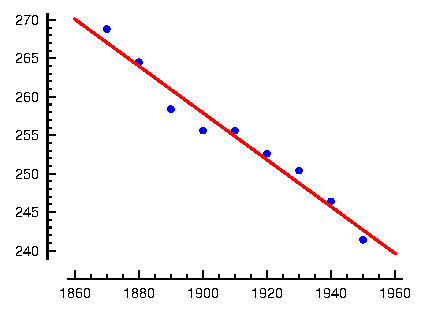
\includegraphics[width=0.5\textwidth]{four_minute_mile.pdf}
\end{center}
Note that the progression is surprisingly linear.
From the slope and intercept we predict $1958.73$; 
the actual date of Roger Bannister's record was 1954-May-06.

The final example
compares team salaries from US major league baseball 
against the number of wins the team had, for the year 2002.
In this year the Oakland Athletics 
used mathematical techniques to optimize the players that they fielded
for the money that they could spend, as told in  
the film \textit{Moneyball}.
(Salaries are in millions of dollars and the number of wins
is out of 180 games). 

To do the computations we use \textit{Sage}. 
% http://ask.sagemath.org/question/768/fitting-a-curve-to-a-straight-line?answer=1271#1271
% by Joaquim Puig on 2011-Sep-27; gathered on 2013-Oct-23 JH
\begin{lstlisting}
sage: sal = [40, 40, 39, 42, 45, 42, 62, 34, 41, 57, 58, 63, 47, 75, 57, 78, 80, 50, 60, 93, 
  77, 55, 95, 103, 79, 76, 108, 126, 95, 106]
sage: wins = [103, 94, 83, 79, 78, 72, 99, 55, 66, 81, 80, 84, 62, 97, 73, 95, 93, 56, 67, 101, 
  78, 55, 92, 98, 74, 67, 93, 103, 75, 72]
sage: var('a, b, t')
(a, b, t)
sage: model(t) = a*t+b
sage: data = zip(sal,wins)
sage: fit = find_fit(data, model, solution_dict=True)
sage: model.subs(fit)
t |--> 0.7447786021698546*t + 7.230396324572004
sage: plot(model.subs(fit),(t,50,110))+points(data,size=25,color='red')
\end{lstlisting}

The graph is below.
The team in the upper left, who paid little for many wins, is
the Oakland A's.

\begin{center}  \small
  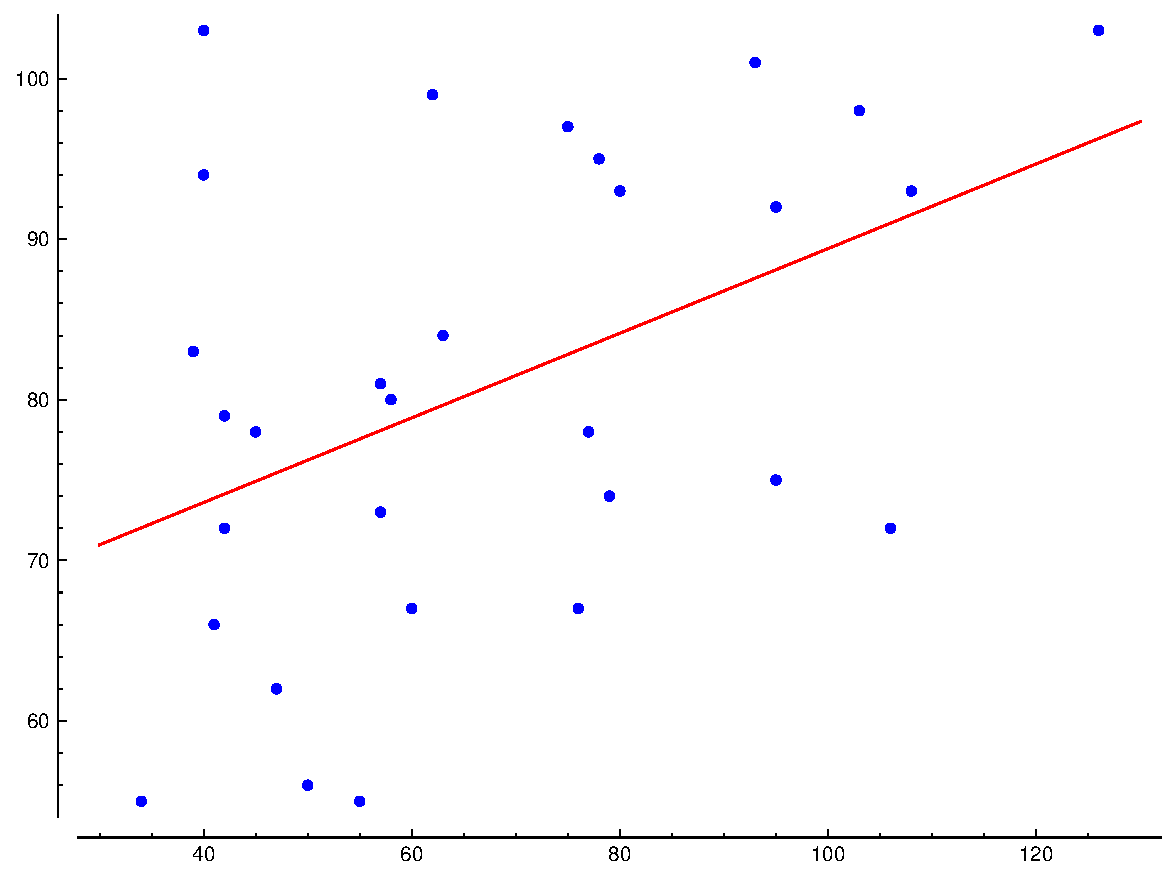
\includegraphics[width=0.5\textwidth]{moneyball.pdf}
\end{center}

Note that in contrast to the penny and mile graphs, 
here judging the line by eye would be error-prone.
So the equations give us a certainty about the `best' in best fit.
In addition, the model's equation tells us roughly that 
by spending an additional million dollars
a team owner could expect to buy $3/4$ of a win.


% For example, the different denominations of US\ money have different average 
% times in circulation.\cite{FedReserve}
% (The $\$2$~bill is a special case because 
% Americans mistakenly believe that 
% it is collectible and do not circulate these bills.)
% \begin{lstlisting}
% sage: x = [1, 5, 10, 20, 50, 100]
% sage: y = [5.9, 4.9, 4.2, 7.7, 3.7, 15.0]
% sage: var('a, b, t') 
% (a, b, t)
% sage: model(t) = a*t+b
% sage: data = zip(x,y)
% sage: fit = find_fit(data, model, solution_dict=True)
% sage: model.subs(fit)                                
% t |--> 0.08650137692301652*t + 4.2184573359365265
% sage: plot(model.subs(fit),(t,0,100))+points(data,size=20,color='red')
% \end{lstlisting}  
% How long should a $\$25$~bill last?

% \begin{center}  \small
%   \includegraphics[width=0.5\textwidth]{denom.png}
% \end{center}


% \begin{center}  \small
%   \begin{tabular}{r|cccccc}
%      \textit{denomination}          
%         &$1$   &$5$    &$10$     &$20$     &$50$     &$100$ \\
%       \hline
%      \textit{average life (mos)}  
%         &$22.0$ &$15.9$  &$18.3$   &$24.3$   &$55.4$   &$88.8$  \\
%   \end{tabular}
% \end{center}
% The data plot below looks roughly linear.
% It isn't a perfect line, i.e.,
% the linear system with equations $b+1m=1.5$, \ldots, $b+100m=20$ has no 
% solution, but we can again use orthogonal projection 
% to find a best approximation.
% Consider the matrix of coefficients of that linear system and also its
% vector of constants, the experimentally-determined values.
% \begin{equation*}
%   A=
%   \begin{mat}[r]
%     1  &1  \\
%     1  &5  \\
%     1  &10  \\
%     1  &20  \\
%     1  &50  \\
%     1  &100  
%   \end{mat}
%   \qquad
%   \vec{v}=\colvec[r]{22.0 \\ 15.9 \\ 18.3 \\ 24.3 \\ 55.4 \\ 88.8}
% \end{equation*}
% The ending result in the subsection on Projection into a Subspace says
% that coefficients $b$ and $m$ so that the linear combination
% of the columns of $A$ is as close as possible to the vector $\vec{v}$ 
% are the entries of $(\trans{A}A)^{-1}\trans{A}\cdot\vec{v}$.
% Some calculation
% gives an intercept of $b=14.16$ and a slope
% of $m= 0.75$.
% \begin{center}  \small
%   \includegraphics{ch3.44}
% \end{center}
% Plugging $x=25$ into the equation of the line shows that such a 
% bill should last about two and three-quarters years.


%
%
%We want to project when a 3:40~mile %\hrsmins{3}{40} 
%will be run.
%\begin{center}
%  \begin{tabular}{r|ccccccc}
%    \textit{year} &1870  &1880  &1890  &1900  &1910  &1920  &1930   \\
%    \hline
%    \textit{secs}  &$268.8$  &$264.5$  &$258.4$  &$255.6$  
%        &$255.6$  &$252.6$  &$250.4$
%  \end{tabular}        \\[2ex]
%  \begin{tabular}{|ccccccc}
%      1940  &1950  &1960  &1970  &1980  &1990 &2000                  \\
%      \hline
%      $246.4$  &$241.4$  &$234.5$  &$231.1$  &$229.0$  &$226.3$ &$223.1$
%  \end{tabular}
%\end{center}
%We can see below that the data is surprisingly linear.
%With this input
%\begin{equation*}
%  A= 
%  \begin{mat}
%    1 & 1860 \\
%    1 & 1870 \\
%%    1 & 1880 \\
%%    1 & 1890 \\ 
%%    1 & 1900 \\ 
%%    1 & 1910 \\
%%    1 & 1920 \\
%%    1 & 1930 \\
%%    1 & 1940 \\
%%    1 & 1950 \\
%%    1 & 1960 \\
%%    1 & 1970 \\
%%    1 & 1980 \\
%    \vdots &\vdots  \\
%    1 &1990  \\
%    1 &2000
%  \end{mat}
%  \qquad
%  \vec{v} = \colvec{280.0 \\
%                    268.8 \\
%%                    264.5 \\
%%                    258.4 \\
%%                    255.6 \\
%%                    255.6 \\
%%                    252.6 \\
%%                    250.4 \\
%%                    246.4 \\
%%                    241.4 \\
%%                    234.5 \\
%%                    231.1 \\
%%                    229.0 \\
%                    \vdots \\
%                    226.3 \\
%                    223.1}
%\end{equation*}
%%MAPLE gives $b=970.68$ and $m=-0.37$  (rounded to two places).
%the Python program at this Topic's end gives 
%%$\text{slope}= -0.351428571429$
%%and $\text{intercept}= 925.534065934$ 
%$\text{slope}= -0.35$
%and $\text{intercept}= 925.53$ 
%(rounded to two places; the original data 
%is good to only about a quarter of a second 
%since much of it was hand-timed).
%\begin{center}  \small
%  \includegraphics{ch3.45}
%\end{center}
%When will a \( 220 \) second mile be run?
%Solving the equation of the line of best fit 
%gives an estimate of the year \( 2008 \).
%
%This example is amusing, but serves as a caution \Dash obviously the 
%linearity of the data will break down someday (as indeed it does 
%prior to 1860).



\begin{exercises}
  \item[]\emph{The calculations here
      are best done on a computer.  
      Some of the problems require more data that is 
      available in your library, on the Internet, 
      or in the Answers to the Exercises.}
  \begin{Filesave}{bookans}  % write the records to the answer file.
    \textit{Data on the progression of the world's records 
       (taken from the \textit{Runner's World} web site)       
       is below.}
    \begin{figure}
      \rotatebox[origin=lb]{90}{\hbox{\scriptsize
        \begin{tabular}[t]{|l|ll|}
%        \hline
%          \multicolumn{3}{|c|}{\textit{Amateurs}}    \\
        \hline
          \multicolumn{3}{|c|}{\textit{Progression of Men's Mile Record}}  \\
        \hline
        \textit{time}  &\textit{name}  &\textit{date}  \\
         \hline  
           $\text{4:52}.0$      &Cadet Marshall (GBR)       &02Sep52 \\
           $\text{4:45}.0$      &Thomas Finch (GBR)         &03Nov58 \\
           %$\text{4:45}.0$      &St.~Vincent Hammick (GBR)  &15Nov58 \\
           $\text{4:40}.0$      &Gerald Surman (GBR)        &24Nov59 \\
           $\text{4:33}.0$      &George Farran (IRL)        &23May62 \\
           $\text{4:29}\;3/5$   &Walter Chinnery (GBR)      &10Mar68 \\
           $\text{4:28}\;4/5$   &William Gibbs (GBR)        &03Apr68 \\ 
           $\text{4:28}\;3/5$   &Charles Gunton (GBR)       &31Mar73 \\
           $\text{4:26}.0$      &Walter Slade (GBR)         &30May74 \\
           $\text{4:24}\;1/2$   &Walter Slade (GBR)         &19Jun75 \\
           $\text{4:23}\;1/5$   &Walter George (GBR)        &16Aug80 \\
           $\text{4:19}\;2/5$   &Walter George (GBR)        &03Jun82 \\
           $\text{4:18}\;2/5$   &Walter George (GBR)        &21Jun84 \\
           $\text{4:17}\;4/5$   &Thomas Conneff (USA)       &26Aug93 \\
           $\text{4:17}.0$      &Fred Bacon (GBR)           &06Jul95 \\
           $\text{4:15}\;3/5$   &Thomas Conneff (USA)       &28Aug95 \\
           $\text{4:15}\;2/5$   &John Paul Jones (USA)      &27May11 \\
           $\text{4:14}.4$      &John Paul Jones (USA)      &31May13 \\
           $\text{4:12}.6$      &Norman Taber (USA)         &16Jul15 \\
           $\text{4:10}.4$      &Paavo Nurmi (FIN)          &23Aug23 \\
           $\text{4:09}\;1/5$   &Jules Ladoumegue (FRA)     &04Oct31 \\
           $\text{4:07}.6$      &Jack Lovelock (NZL)        &15Jul33 \\
           $\text{4:06}.8$      &Glenn Cunningham (USA)     &16Jun34 \\
           $\text{4:06}.4$      &Sydney Wooderson (GBR)     &28Aug37 \\
           $\text{4:06}.2$      &Gunder Hagg (SWE)          &01Jul42 \\
           %$\text{4:06}.2$      &Arne Andersson (SWE)       &10Jul42 \\
           $\text{4:04}.6$      &Gunder Hagg (SWE)          &04Sep42 \\
           $\text{4:02}.6$      &Arne Andersson (SWE)       &01Jul43 \\
           $\text{4:01}.6$      &Arne Andersson (SWE)       &18Jul44 \\
           $\text{4:01}.4$      &Gunder Hagg (SWE)          &17Jul45 \\
           $\text{3:59}.4$      &Roger Bannister (GBR)      &06May54 \\
           $\text{3:58}.0$      &John Landy (AUS)           &21Jun54 \\
           $\text{3:57}.2$      &Derek Ibbotson (GBR)       &19Jul57 \\
           $\text{3:54}.5$      &Herb Elliott (AUS)         &06Aug58 \\
           $\text{3:54}.4$      &Peter Snell (NZL)          &27Jan62 \\ 
           $\text{3:54}.1$      &Peter Snell (NZL)          &17Nov64 \\
           $\text{3:53}.6$      &Michel Jazy (FRA)          &09Jun65 \\
           $\text{3:51}.3$      &Jim Ryun (USA)             &17Jul66 \\
           $\text{3:51}.1$      &Jim Ryun (USA)             &23Jun67 \\
           $\text{3:51}.0$      &Filbert Bayi (TAN)         &17May75 \\
           $\text{3:49}.4$      &John Walker (NZL)          &12Aug75 \\
           $\text{3:49}.0$      &Sebastian Coe (GBR)        &17Jul79 \\
           $\text{3:48}.8$      &Steve Ovett (GBR)          &01Jul80 \\
           $\text{3:48}.53$     &Sebastian Coe (GBR)        &19Aug81 \\
           $\text{3:48}.40$     &Steve Ovett (GBR)          &26Aug81 \\
           $\text{3:47}.33$     &Sebastian Coe (GBR)        &28Aug81 \\
           $\text{3:46}.32$     &Steve Cram (GBR)           &27Jul85 \\
           $\text{3:44}.39$     &Noureddine Morceli (ALG)   &05Sep93 \\
	   $\text{3:43}.13$     &Hicham el Guerrouj (MOR)   &07Jul99 \\
      \hline
      \end{tabular}
      \   %
        \begin{tabular}[t]{|l|ll|}
        \hline
          \multicolumn{3}{|c|}{\textit{Progression of Men's $1500$~Meter Record}}  \\
        \hline
        \textit{time}  &\textit{name}  &\textit{date}  \\
         \hline  
         $\text{4:09}.0$   &John Bray (USA)        &30May00  \\
         $\text{4:06}.2$   &Charles Bennett (GBR)  &15Jul00  \\
         $\text{4:05}.4$   &James Lightbody (USA)  &03Sep04  \\
         $\text{3:59}.8$   &Harold Wilson (GBR)    &30May08  \\
         $\text{3:59}.2$   &Abel Kiviat (USA)      &26May12  \\
         $\text{3:56}.8$   &Abel Kiviat (USA)      &02Jun12  \\
         $\text{3:55}.8$   &Abel Kiviat (USA)      &08Jun12  \\
         $\text{3:55}.0$   &Norman Taber (USA)     &16Jul15  \\
         $\text{3:54}.7$   &John Zander (SWE)      &05Aug17  \\
         $\text{3:53}.0$   &Paavo Nurmi (FIN)      &23Aug23  \\
         $\text{3:52}.6$   &Paavo Nurmi (FIN)      &19Jun24  \\
         $\text{3:51}.0$   &Otto Peltzer (GER)     &11Sep26  \\
         $\text{3:49}.2$   &Jules Ladoumegue (FRA) &05Oct30  \\
         %$\text{3:49}.2$   &Luigi Beccali (ITA)    &09Sep33  \\
         $\text{3:49}.0$   &Luigi Beccali (ITA)    &17Sep33  \\
         $\text{3:48}.8$   &William Bonthron (USA) &30Jun34  \\
         $\text{3:47}.8$   &Jack Lovelock (NZL)    &06Aug36  \\
         $\text{3:47}.6$   &Gunder Hagg (SWE)      &10Aug41  \\
         $\text{3:45}.8$   &Gunder Hagg (SWE)      &17Jul42  \\
         $\text{3:45}.0$   &Arne Andersson (SWE)   &17Aug43  \\
         $\text{3:43}.0$   &Gunder Hagg (SWE)      &07Jul44  \\
         %$\text{3:43}.0$   &Lennart Strand (SWE)   &15Jul47  \\
         %$\text{3:43}.0$   &Werner Lueg (FRG)      &29Jun52  \\
         %$\text{3:43}.0$   &Roger Bannister (GBR)  &06May54  \\
         $\text{3:42}.8$   &Wes Santee (USA)       &04Jun54  \\
         $\text{3:41}.8$   &John Landy (AUS)       &21Jun54  \\
         $\text{3:40}.8$   &Sandor Iharos (HUN)    &28Jul55  \\
         %$\text{3:40}.8$   &Laszlo Tabori (HUN)    &06Sep55  \\
         %$\text{3:40}.8$   &Gunnar Nielsen (DEN)   &06Sep55  \\
         $\text{3:40}.6$   &Istvan Rozsavolgyi (HUN) &03Aug56 \\
         $\text{3:40}.2$   &Olavi Salsola (FIN)    &11Jul57  \\
         %$\text{3:40}.2$   &Olavi Salonen (FIN)    &11Jul57  \\
         $\text{3:38}.1$   &Stanislav Jungwirth (CZE) &12Jul57  \\
         $\text{3:36}.0$   &Herb Elliott (AUS)     &28Aug58  \\
         $\text{3:35}.6$   &Herb Elliott (AUS)     &06Sep60  \\
         $\text{3:33}.1$   &Jim Ryun (USA)         &08Jul67  \\
         $\text{3:32}.2$   &Filbert Bayi (TAN)     &02Feb74  \\
         $\text{3:32}.1$   &Sebastian Coe (GBR)    &15Aug79  \\
         %$\text{3:32}.1$   &Steve Ovett (GBR)      &15Jul80  \\  
         $\text{3:31}.36$  &Steve Ovett (GBR)      &27Aug80  \\
         $\text{3:31}.24$  &Sydney Maree (usa)     &28Aug83  \\
         $\text{3:30}.77$  &Steve Ovett (GBR)      &04Sep83  \\
         $\text{3:29}.67$  &Steve Cram (GBR)       &16Jul85  \\
         $\text{3:29}.46$  &Said Aouita (MOR)      &23Aug85  \\ 
         $\text{3:28}.86$  &Noureddine Morceli (ALG)  &06Sep92  \\
         $\text{3:27}.37$  &Noureddine Morceli (ALG)  &12Jul95  \\
         $\text{3:26}.00$  &Hicham el Guerrouj (MOR)  &14Jul98  \\
     \hline
     \end{tabular}
      \   %
        \begin{tabular}[t]{|l|ll|}
        \hline
          \multicolumn{3}{|c|}{\textit{Progression of Women's Mile Record}}  \\
        \hline
        \textit{time}  &\textit{name}  &\textit{date}  \\
         \hline  
           $\text{6:13}.2$    &Elizabeth Atkinson (GBR)    &24Jun21 \\
           $\text{5:27}.5$    &Ruth Christmas (GBR)        &20Aug32 \\
           $\text{5:24}.0$    &Gladys Lunn (GBR)           &01Jun36 \\
           $\text{5:23}.0$    &Gladys Lunn (GBR)           &18Jul36 \\
           $\text{5:20}.8$    &Gladys Lunn (GBR)           &08May37 \\
           $\text{5:17}.0$    &Gladys Lunn (GBR)           &07Aug37 \\
           $\text{5:15}.3$    &Evelyne Forster (GBR)       &22Jul39 \\
           $\text{5:11}.0$    &Anne Oliver (GBR)           &14Jun52 \\
           $\text{5:09}.8$    &Enid Harding (GBR)          &04Jul53 \\
           $\text{5:08}.0$    &Anne Oliver (GBR)           &12Sep53 \\
           $\text{5:02}.6$    &Diane Leather (GBR)         &30Sep53 \\
           $\text{5:00}.3$    &Edith Treybal (ROM)         &01Nov53 \\
           $\text{5:00}.2$    &Diane Leather (GBR)         &26May54 \\
           $\text{4:59}.6$    &Diane Leather (GBR)         &29May54 \\
           $\text{4:50}.8$    &Diane Leather (GBR)         &24May55 \\
           $\text{4:45}.0$    &Diane Leather (GBR)         &21Sep55 \\
           $\text{4:41}.4$    &Marise Chamberlain (NZL)    &08Dec62 \\
           $\text{4:39}.2$    &Anne Smith (GBR)            &13May67 \\
           $\text{4:37}.0$    &Anne Smith (GBR)            &03Jun67 \\
           $\text{4:36}.8$    &Maria Gommers (HOL)         &14Jun69 \\
           $\text{4:35}.3$    &Ellen Tittel (FRG)          &20Aug71 \\
           $\text{4:34}.9$    &Glenda Reiser (CAN)         &07Jul73 \\
           $\text{4:29}.5$    &Paola Pigni-Cacchi (ITA)    &08Aug73 \\
           $\text{4:23}.8$    &Natalia Marasescu (ROM)     &21May77 \\
           $\text{4:22}.1$    &Natalia Marasescu (ROM)     &27Jan79 \\
           $\text{4:21}.7$    &Mary Decker (USA)           &26Jan80 \\
           $\text{4:20}.89$   &Lyudmila Veselkova (SOV)    &12Sep81 \\
           $\text{4:18}.08$   &Mary Decker-Tabb (USA)      &09Jul82 \\
           $\text{4:17}.44$   &Maricica Puica (ROM)        &16Sep82 \\
           $\text{4:15}.8$    &Natalya Artyomova (SOV)     &05Aug84 \\
           $\text{4:16}.71$   &Mary Decker-Slaney (USA)    &21Aug85 \\
           $\text{4:15}.61$   &Paula Ivan (ROM)            &10Jul89 \\
           $\text{4:12}.56$   &Svetlana Masterkova (RUS)   &14Aug96 \\
       \hline
       \end{tabular}
      }}  %end the rotatebox
    \end{figure}
  \end{Filesave}  
  \item
    Use least-squares to judge if the coin in this experiment is fair.
    \begin{center}
      \begin{tabular}{r|ccccc}
         \textit{flips}  &8  &16  &24  &32  &40 \\
         \hline
         \textit{heads}  &4  &9   &13  &17  &20
      \end{tabular}
    \end{center}
    \begin{answer}
      As with the first example discussed above, we are trying to find a 
      best $m$ to ``solve'' this system. 
      \begin{equation*}
        \begin{linsys}{5}
          8m  &=  &4  \\
          16m &=  &9  \\
          24m &=  &13 \\
          32m &=  &17 \\
          40m &=  &20
        \end{linsys}
      \end{equation*}
      Projecting into the linear subspace gives this
      \begin{equation*}
        \frac{\colvec[r]{4 \\ 9 \\ 13 \\ 17 \\20}
          \dotprod
          \colvec[r]{8  \\ 16 \\ 24 \\ 32 \\ 40}}{%
          \colvec[r]{8  \\ 16 \\ 24 \\ 32 \\ 40}
          \dotprod
          \colvec[r]{8  \\ 16 \\ 24 \\ 32 \\ 40}}
        \cdot
        \colvec[r]{8  \\ 16 \\ 24 \\ 32 \\ 40}
        =
        \frac{1832}{3520}
        \cdot
        \colvec[r]{8  \\ 16 \\ 24 \\ 32 \\ 40}
      \end{equation*}
      so the slope of the line of best fit is approximately $0.52$.
      \begin{center}  \small
        \includegraphics{ch3.85}
      \end{center}
    \end{answer}
  \item 
     For the men's mile record, rather than give each of the many 
     records and its exact date, we've ``smoothed'' the data somewhat by 
     taking a periodic sample.
     Do the longer calculation and compare the conclusions.
     \begin{answer}
     With this input
     \begin{equation*}
       A =  
       \begin{mat}
           1 & 1852.71 \\
           1 & 1858.88 \\
          \vdots  &\vdots      \\
           1 & 1985.54 \\
           1 & 1993.71
        \end{mat}
        \qquad
        b = \colvec{ 292.0 \\ 
                     285.0 \\ 
                    \vdots  \\
                     226.32 \\
                     224.39}
     \end{equation*}
     (the dates have been rounded to months, e.g., for a September record,
     the decimal $.71\approx (8.5/12)$ was used), Maple responded
     with an intercept of $b=994.8276974$ and a slope of
     $m=-0.3871993827$.    
     \begin{center}  \small
        \includegraphics{ch3.86}
     \end{center}
     \end{answer}
  \item 
    Find the line of best fit for the men's $1500$~meter run.
    How does the slope compare with that for the men's mile?
    (The distances are close; a mile is about $1609$~meters.)
    \begin{answer}
   With this input (the years are zeroed at $1900$)
   \begin{equation*}
     A := 
     \begin{mat}
        1 &   .38   \\
        1 &   .54   \\
       \vdots \vdots \\ 
        1 & 92.71 \\
        1 & 95.54
     \end{mat}
     \qquad      
     b = \colvec{ 249.0 \\
                  246.2 \\
                 \vdots \\
                  208.86 \\
                  207.37}
   \end{equation*}
     (the dates have been rounded to months, e.g., for a September record,
     the decimal $.71\approx (8.5/12)$ was used),   
     Maple gives an intercept of $b=243.1590327$ and a slope of 
   $m=-0.401647703$.
   The slope given in the body of this Topic for the men's mile is 
   quite close to this.
   \begin{center}  \small
     \includegraphics{ch3.87}
   \end{center}
   \end{answer}
  \item Find the line of best fit for the records for women's mile.
    \begin{answer}
    With this input (the years are zeroed at $1900$)
    \begin{equation*}
      A =  
      \begin{mat}
         1 & 21.46 \\
         1 & 32.63 \\
        \vdots  &\vdots     \\
         1 & 89.54  \\
         1 & 96.63
      \end{mat}
      \qquad
      b = 
      \colvec{ 373.2 \\
               327.5 \\
              \vdots  \\
               255.61 \\
               252.56}      
    \end{equation*}
     (the dates have been rounded to months, e.g., for a September record,
     the decimal $.71\approx (8.5/12)$ was used),
     MAPLE gave an intercept of $b=378.7114894$ and a slope of 
    $m=-1.445753225$.
    \begin{center}  \small
      \includegraphics{ch3.88}
    \end{center}
   \end{answer}   
  \item 
  Do the lines of best fit for the men's and women's miles cross?
  \begin{answer}
    These are the equations of the lines for men's and women's mile 
    (the vertical intercept term of the equation
    for the women's mile has been adjusted from the answer above,
    to zero it at the year $0$,
    because that's how the men's mile equation was done).
    \begin{align*}
        y &=994.8276974-0.3871993827x  \\
        y &=3125.6426-1.445753225x
    \end{align*}
    Obviously the lines cross.
    A computer program  is the easiest way to do the
    arithmetic:~MuPAD gives $x=2012.949004$ and $y=215.4150856$
    ($215$~seconds is $3$~minutes and $35$~seconds).
    \textit{Remark.}
    Of course all of this projection is highly dubious \Dash  for one thing,
    the equation for the women is influenced by the quite slow early 
    times \Dash  but it is nonetheless fun.
     \begin{center}  \small
       \includegraphics{ch3.89}
     \end{center}
  \end{answer}
%  \item 
%     Look up the records for the men's and women's marathon.
%     Find the line of best fit for each.
%     Do the lines cross?
%  \item 
%    Look up the records for men's long jump.
%    How far out-of-trend was Bob Beamon's record?
  \item
    \textit{(This illustrates that there are data sets for which a 
    linear model is not right,  and that the line of best fit doesn't
    in that case have any predictive value.)} 
    In a highway restaurant a trucker told me that his boss often sends 
    him by a roundabout route, using more gas
    but paying lower bridge tolls.
    He said that New York State calibrates the 
    toll for each bridge across the Hudson, 
    playing off the extra gas to get there
    from New York City against a lower crossing cost,
    to encourage people to go upstate.
    This table, from \cite{CostOfTolls} and \cite{GoogleMaps},
    lists for each toll crossing of the Hudson River, 
    the distance to drive from Times Square in miles and the cost in US~dollars 
    for a passenger car
    (if a crossings has a one-way toll then it shows half that number). 
    \begin{center}
      \small
      % \begin{tabular}{lrr}
      %    \multicolumn{1}{c}{\textit{Crossing}}
      %      &\multicolumn{1}{c}{\textit{Distance}}
      %      &\textit{Toll}  \\ \hline
      %    Lincoln Tunnel &$2$  &$6.00$ \\
      %    Holland Tunnel &$7$  &$6.00$  \\
      %    George Washington Bridge &$8$  &$6.00$  \\
      %    Verrazano-Narrows Bridge &$16$  &$6.50$  \\
      %    Tappan Zee Bridge &$27$  &$2.50$  \\
      %    Bear Mountain Bridge &$47$  &$1.00$  \\
      %    Newburgh-Beacon Bridge &$67$  &$1.00$  \\
      %    Mid-Hudson Bridge &$82$  &$1.00$  \\
      %    Kingston-Rhinecliff Bridge &$102$  &$1.00$  \\
      %    Rip Van Winkle Bridge &$120$  &$1.00$  
      % \end{tabular}
      \begin{tabular}{ccc}
         \textit{Crossing}
           &\textit{Distance}
           &\textit{Toll}  \\ \hline
         \begin{tabular}{@{}l@{}}
           Lincoln Tunnel \\
           Holland Tunnel  \\
           George Washington Bridge  \\
           Verrazano-Narrows Bridge   \\
           Tappan Zee Bridge  \\
           Bear Mountain Bridge  \\
           Newburgh-Beacon Bridge  \\
           Mid-Hudson Bridge   \\
           Kingston-Rhinecliff Bridge  \\
           Rip Van Winkle Bridge   
         \end{tabular}
         &\begin{tabular}{@{}r@{}}
           $2$ \\
           $7$  \\
           $8$  \\
           $16$  \\
           $27$   \\
           $47$   \\
           $67$   \\
           $82$  \\
           $102$  \\
           $120$ 
          \end{tabular}  
         &\begin{tabular}{@{}r@{}}
           $6.00$ \\
           $6.00$  \\
           $6.00$  \\
           $6.50$  \\
           $2.50$  \\
           $1.00$  \\
           $1.00$  \\
           $1.00$  \\
           $1.00$  \\
           $1.00$ 
         \end{tabular} 
      \end{tabular}
    \end{center}
    Find the line of best fit and graph the data to
    show that the driver was practicing on my credulity.
    \begin{answer}
      \textit{Sage} gives the line of best fit as
      $\text{toll}=-0.05\text{dist}+5.63$.
      But the graph shows that the equation has no predictive value.
      \begin{center}
        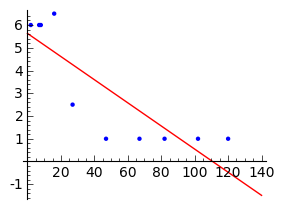
\includegraphics{bridges.png}
      \end{center}
      Apparently a better model is that 
      (with only one intermediate exception) crossings in the city
      cost roughly the same as each other,
      and crossings upstate cost the same as each other.
    \end{answer}
  \item 
    When the space shuttle Challenger exploded in 1986, one of the
    criticisms made of NASA's decision to launch was in the way they did the
    analysis of number of O-ring failures versus temperature
    (O-ring failure caused the explosion).
    Four O-ring failures would be fatal.
    NASA had data from $24$ previous flights.
    \begin{center}
      \begin{tabular}{r|rrrrrrrrrrr}
         \textit{temp\ ${}^\circ$F} 
            &53 &75 &57 &58 &63 &70 &70 &66 &67 &67 &67 \\
         \hline
         \textit{failures}  
            &3  &2  &1  &1  &1  &1  &1  &0  &0  &0  &0
      \end{tabular}\hspace*{3em}                                           \\
      \hspace*{3em}\begin{tabular}{|rrrrrrrrrrrrr}
                68 &69 &70 &70 &72 &73 &75 &76 &76 &78 &79 &80 &81\\
         \hline
                0  &0  &0  &0  &0  &0  &0  &0  &0  &0  &0  &0  &0
      \end{tabular}
    \end{center}
    The temperature that day was forecast to be \( 31^\circ\text{F} \).
    \begin{exparts}
      \partsitem NASA based the decision to launch partially on a chart showing
        only the flights that had at least one O-ring failure.
        Find the line that best fits these seven flights.
        On the basis of this data,
        predict the number of O-ring failures when the temperature is $31$, and
        when the number of failures will exceed four.
      \partsitem Find the line that best fits all 24 flights.
        On the basis of this extra data,
        predict the number of O-ring failures when the temperature is $31$, and
        when the number of failures will exceed four.
    \end{exparts}
    Which do you think is the more accurate method of predicting?
    (An excellent discussion is in \cite{Stats}.)
    \begin{answer}
      \begin{exparts}
        \partsitem A computer algebra system like MAPLE or MuPAD will give
          an intercept of $b=4259/1398\approx 3.239628$
          and a slope of $m=-71/2796\approx -0.025393419$     
          Plugging $x=31$ into the equation yields a predicted number of
          O-ring failures of $y=2.45$ (rounded to two places).
          Plugging in $y=4$ and solving gives a temperature of
          $x=-29.94^\circ$F.
        \partsitem On the basis of this information
          \begin{equation*}
            A =  
            \begin{mat}
               1 & 53 \\
               1 & 75 \\
%              1 & 57 \\
%              1 & 58 \\
%              1 & 63 \\
%              1 & 70 \\
%              1 & 70 \\
%              1 & 66 \\
%              1 & 67 \\
%              1 & 67 \\
%              1 & 67 \\
%              1 & 68 \\
%              1 & 69 \\
%              1 & 70 \\
%              1 & 70 \\
%              1 & 72 \\
%              1 & 73 \\
%              1 & 75 \\
%              1 & 76 \\
%              1 & 76 \\
%              1 & 78 \\
%              1 & 79 \\
               \vdots \\
               1 & 80 \\
               1 & 81
            \end{mat}
            \qquad
            b = 
            \colvec{ 3 \\
                     2 \\
%                    1 \\
%                    1 \\
%                    1 \\
%                    1 \\
%                    1 \\
%                    0 \\ 
%                    0 \\
%                    0 \\
%                    0 \\
%                    0 \\
%                    0 \\
%                    0 \\
%                    0 \\
%                    0 \\
%                    0 \\
%                    0 \\
%                    0 \\
%                    0 \\
%                    0 \\
%                    0 \\
                     \vdots \\
                     0 \\
                     0}
          \end{equation*}
          MAPLE gives the intercept $b=187/40=4.675$ and the 
          slope $m=-73/1200\approx -0.060833$.
          Here, plugging $x=31$ into the equation predicts 
          $y=2.79$ O-ring failures (rounded to two places).
          Plugging in $y=4$~failures gives a temperature of 
          $x=11^\circ$F.
     \begin{center}  \small
       \includegraphics{ch3.90}
      \end{center}
      \end{exparts}  
    \end{answer}
  \item 
     This table lists the average distance from the sun to
     each of the first seven planets, using Earth's average as a unit.
     \begin{center}
       \begin{tabular}{ccccccc}
         Mercury &Venus   &Earth   &Mars    &Jupiter &Saturn  &Uranus  \\ 
         \hline     
         $0.39$  &$0.72$  &$1.00$  &$1.52$  &$5.20$  &$9.54$  &$19.2$
       \end{tabular}
     \end{center}
    \begin{exparts}
      \partsitem Plot the number of the planet 
        (Mercury is \( 1 \), etc.) versus the distance.
        Note that it does not look like a line, and so finding the
        line of best fit is not fruitful.
      \partsitem It does, however look like an exponential curve. 
        Therefore, plot the number of the planet versus the
        logarithm of the distance.
        Does this look like a line?
      \partsitem The asteroid belt between Mars and
        Jupiter is 
        what is left of a planet that broke apart.
        Renumber so that Jupiter is $6$, Saturn is $7$, and Uranus is
        $8$, and plot against the log again.
        Does this look better?
      \partsitem Use least squares on that data to predict the 
       location of Neptune.
      \partsitem Repeat to predict where Pluto is.
      \partsitem Is the formula accurate for Neptune and Pluto? 
    \end{exparts}
    This method was used to help discover Neptune (although the second item is
    misleading about the history; actually, the discovery of Neptune 
    in position~$9$ 
    prompted people to look for the ``missing planet'' in position~$5$).
    See \cite{Gardner70}
      \begin{answer}
        \begin{exparts}
          \partsitem The plot is nonlinear.
            \begin{center}  \small
              \includegraphics{ch3.91}
            \end{center}
          \partsitem Here is the plot.
           \begin{center}  \small
             \includegraphics{ch3.92}
           \end{center}
           There is perhaps a jog up between planet~$4$ and planet~$5$.
          \partsitem This plot seems even more linear.
           \begin{center}  \small
             \includegraphics{ch3.93}
           \end{center}
          \partsitem
            With this input
            \begin{equation*}
              A =  
              \begin{mat}[r]
                1 & 1 \\
                1 & 2 \\
                1 & 3 \\
                1 & 4 \\
                1 & 6 \\
                1 & 7 \\
                1 & 8
              \end{mat}
              \qquad
              b = \colvec[r]{-0.40893539 \\
                          -0.1426675 \\
                           0 \\
                           0.18184359 \\
                           0.71600334 \\
                           0.97954837 \\
                           1.2833012}
            \end{equation*}
            MuPAD gives that the intercept is $b= -0.6780677466$ and
            the slope is $m=0.2372763818$.
          \partsitem Plugging $x=9$ into the equation
            $y= -0.6780677466+0.2372763818x$ from the prior item gives
            that the log of the distance is $1.4574197$, so the expected
            distance is $28.669472$.
            The actual distance is about $30.003$.
          \partsitem Plugging $x=10$ into the same equation
            gives that the log of the distance is $1.6946961$, so the expected
            distance is $49.510362$.
            The actual distance is about $39.503$.
        \end{exparts}
      \end{answer}
  % \item 
  %   William Bennett has proposed an Index of Leading Cultural Indicators
  %   for the US (\cite{Bennett}, in 1993).
  %   Among the statistics cited are the average daily hours spent watching TV, 
  %   and the average combined SAT scores.
  %   \begin{center}
  %     \begin{tabular}{r|cccccccc}
  %        &1960   &1965   &1970   &1975   &1980   &1985   &1990   &1992  
  %           \\ \hline
  %        \textit{TV}
  %        &5:06   &5:29   &5:56   &6:07   &6:36   &7:07   &6:55   &7:04 \\
  %        \textit{SAT}
  %        &$975$  &$969$  &$948$  &$910$  &$890$  &$906$  &$900$  &$899$ 
  %     \end{tabular} 
  %   \end{center}
  %   Suppose that a cause and effect relationship is proposed between
  %   the time spent watching TV and the decline in SAT scores (in this article,
  %   Mr.~Bennett does not argue that there is a direct connection).
  %   \begin{exparts}
  %    \partsitem Find the line of best fit relating the independent variable
  %      of average daily TV hours to the dependent variable of SAT scores.
  %    \partsitem Find the most recent estimate of the average daily TV hours  
  %      (Bennett's cites Neilsen Media Research as the source of these 
  %      estimates).
  %      Estimate the associated SAT score.
  %      How close is your estimate to the actual average?
  %      (Warning: a change has been made recently in the SAT,
  %      so you should investigate whether some adjustment needs to be made to
  %      the reported average to make a valid comparison.)
  %   \end{exparts}
  %   \begin{answer}
  %     \begin{exparts}
  %       \partsitem With this input
  %         \begin{equation*}
  %           A = 
  %           \begin{mat}[r]
  %             1 & 306 \\
  %             1 & 329 \\
  %             1 & 356 \\
  %             1 & 367 \\
  %             1 & 396 \\
  %             1 & 427 \\
  %             1 & 415 \\
  %             1 & 424
  %           \end{mat}
  %           \qquad
  %           b = 
  %           \colvec[r]{975 \\
  %                   969 \\
  %                   948 \\
  %                   910 \\
  %                   890 \\
  %                   906 \\
  %                   900 \\
  %                   899}
  %         \end{equation*}
  %         MAPLE gives the intercept 
  %         $b=34009779/28796\approx 1181.0591$ and the slope 
  %         $m=-19561/28796\approx -0.6793$.
  %         \begin{center}  \small
  %           \includegraphics{ch3.94}
  %      \end{center}
  %     \end{exparts}
  %   \end{answer}
%  \item
%    Derive the 
%    \definend{normal equations}\index{least squares!normal equations}%
%    \index{normal equations!for least squares} for least squares line fitting:
%    for data points \( (x_1,y_1) \), \ldots, \( (x_n,y_n) \)
%    the line of best fit \( y=mx+b \) has this slope
%    \begin{equation*}
%      m=\frac{\frac{\displaystyle x_1y_1+\dots+x_ny_n}{\displaystyle n}
%              -(\frac{\displaystyle x_1+\dots+x_n}{\displaystyle n})
%               (\frac{\displaystyle y_1+\dots+y_n}{\displaystyle n})}{
%              \frac{\displaystyle {x_1}^2+\cdots+{x_n}^2}{\displaystyle n}
%              -(\frac{\displaystyle x_1+\dots+x_n}{\displaystyle n})^2}
%    \end{equation*}
%    and this vertical intercept.
%    \begin{equation*}
%      b=\frac{y_1+\dots+y_n}{n}-m(\frac{x_1+\dots+x_n}{n})
%    \end{equation*}
%    (\textit{Remark}.
%     A advantage of these equations is that a
%     person doing by-hand calculations can make up \Dash  and check \Dash  a 
%     table with a
%     column of $x_i$'s, one of $y_i$'s, one of $x_i^2$'s,
%     one of $y_i^2$'s , and finally one of $x_i\cdot y_i$'s.
%     Then the sums of these columns fit into the formulas.)
%     \begin{answer}
%       The $\nbyn{2}$ shows how the larger cases hold.
%     \end{answer}
\end{exercises}
%\par\noindent\announcecomputercode %
%\begin{computercode}
%    #!/usr/bin/python
%    # least_squares.py   calculate the line of best fit for a data set
%    # data file format: each line is two numbers, x and y
%    import math, string
%
%    n = 0
%    sum__x = 0
%    sum_y = 0
%    sum_x_squared = 0
%    sum_xy = 0
%
%    fn = raw_input("Name of the data file? ")
%    datafile = open(fn,"r")
%    while 1:
%      ln = datafile.readline()
%      if (ln):
%            data = string.split(ln)
%            x = string.atof(data[0])
%            y = string.atof(data[1])
%            n = n+1
%            sum_x = sum_x+x
%            sum_y = sum_y+y
%            sum_x_squared = sum_x_squared+(x*x)
%            sum_xy = sum_xy +(x*y)
%      else:
%            break
%    datafile.close()
%
%    slope=(sum_of_xy-pow(sum_x,2)/n)/(sum_x_squared-pow(sum_x,2)/n)
%    intercept=(sum_y-(slope*sum_x))/n
%    print "line of best fit: slope=",slope," intercept=",intercept 
%\end{computercode}


\index{line of best fit|)}
\index{least squares|)}






